\documentclass[a4paper,oneside,14pt]{extarticle}

\usepackage{cmap} % Улучшенный поиск русских слов в полученном pdf-файле
\usepackage[T2A]{fontenc} % Поддержка русских букв
\usepackage[utf8]{inputenc} % Кодировка utf8
\usepackage[english,russian]{babel} % Языки: русский, английский

\usepackage[14pt]{extsizes}

\usepackage{graphicx}
\usepackage{multirow}

\usepackage{tikz}
\usetikzlibrary{shapes, shapes.geometric, arrows, arrows.meta, positioning}

\usepackage{caption}
\captionsetup{labelsep=endash}
\captionsetup[figure]{name={Рисунок}}

\usepackage{amsmath}
\usepackage{amsfonts}

\usepackage{geometry}
\geometry{left=30mm}
\geometry{right=10mm}
\geometry{top=20mm}
\geometry{bottom=20mm}

\usepackage{enumitem}

\usepackage{tabularx}
\usepackage{longtable}
\usepackage{adjustbox}
\usepackage{threeparttable}

% Переопределение стандартных \section, \subsection, \subsubsection по ГОСТу;
\usepackage{titlesec}[explicit]
\titleformat{name=\section,numberless}[block]{\normalfont\large\bfseries\centering}{}{0pt}{}
\titleformat{\section}[block]{\normalfont\large\bfseries}{\thesection}{1em}{}
\titlespacing\section{\parindent}{*4}{*4}

\titleformat{\subsection}[hang]
{\bfseries\large}{\thesubsection}{1em}{}
\titlespacing\subsection{\parindent}{*2}{*2}

\titleformat{\subsubsection}[hang]
{\bfseries\large}{\thesubsubsection}{1em}{}
\titlespacing\subsubsection{\parindent}{*2}{*2}

\usepackage{url}

% Переопределение их отступов до и после для 1.5 интервала во всем документе
\usepackage{setspace}
\onehalfspacing % Полуторный интервал
\frenchspacing
\setlength\parindent{1.25cm}

\usepackage{indentfirst} % Красная строка

% Настройки оглавления
\usepackage{xcolor}
\usepackage{multirow}

% Гиперссылки
\usepackage[pdftex]{hyperref}
\hypersetup{hidelinks}

% Дополнительное окружения для подписей
\usepackage{array}
\newenvironment{signstabular}[1][1]{
	\renewcommand*{\arraystretch}{#1}
	\tabular
}{
	\endtabular
}

\usepackage{enumitem} 
\setenumerate[0]{label=\arabic*)} % Изменение вида нумерации списков
\renewcommand{\labelitemi}{---}

% Листинги 
\usepackage{courier}
\usepackage{listings}
\usepackage{chngcntr} % Listings counter within section set main.tex after begin document
\usepackage{float} % Place figures anywhere you want; ignore floating
\floatstyle{plaintop}
\newfloat{code}{H}{myc}

% Для листинга кода:
\lstset{
	basicstyle=\small\ttfamily,
	language=prolog,
	numbers=left,
	numbersep=5pt,
	% stepnumber=1,
	xleftmargin=17pt,
	% showstringspaces=false,
	numbersep=5pt,
	frame=single,
	tabsize=4,
	captionpos=b,
	breaklines=true,
	breakatwhitespace=true,
	escapeinside={\#*}{*)},
	inputencoding=utf8x,
	backgroundcolor=\color{white},
	% numberstyle=,%\tiny
	keywordstyle=\color{blue},
	stringstyle=\color{red!90!black},
	commentstyle=\color{green!50!black}
}
\lstset{
 morekeywords={domains, predicates, clauses, goal}
}

\lstset{
	literate=
	{а}{{\selectfont\char224}}1
	{б}{{\selectfont\char225}}1
	{в}{{\selectfont\char226}}1
	{г}{{\selectfont\char227}}1
	{д}{{\selectfont\char228}}1
	{е}{{\selectfont\char229}}1
	{ё}{{\"e}}1
	{ж}{{\selectfont\char230}}1
	{з}{{\selectfont\char231}}1
	{и}{{\selectfont\char232}}1
	{й}{{\selectfont\char233}}1
	{к}{{\selectfont\char234}}1
	{л}{{\selectfont\char235}}1
	{м}{{\selectfont\char236}}1
	{н}{{\selectfont\char237}}1
	{о}{{\selectfont\char238}}1
	{п}{{\selectfont\char239}}1
	{р}{{\selectfont\char240}}1
	{с}{{\selectfont\char241}}1
	{т}{{\selectfont\char242}}1
	{у}{{\selectfont\char243}}1
	{ф}{{\selectfont\char244}}1
	{х}{{\selectfont\char245}}1
	{ц}{{\selectfont\char246}}1
	{ч}{{\selectfont\char247}}1
	{ш}{{\selectfont\char248}}1
	{щ}{{\selectfont\char249}}1
	{ъ}{{\selectfont\char250}}1
	{ы}{{\selectfont\char251}}1
	{ь}{{\selectfont\char252}}1
	{э}{{\selectfont\char253}}1
	{ю}{{\selectfont\char254}}1
	{я}{{\selectfont\char255}}1
	{А}{{\selectfont\char192}}1
	{Б}{{\selectfont\char193}}1
	{В}{{\selectfont\char194}}1
	{Г}{{\selectfont\char195}}1
	{Д}{{\selectfont\char196}}1
	{Е}{{\selectfont\char197}}1
	{Ё}{{\"E}}1
	{Ж}{{\selectfont\char198}}1
	{З}{{\selectfont\char199}}1
	{И}{{\selectfont\char200}}1
	{Й}{{\selectfont\char201}}1
	{К}{{\selectfont\char202}}1
	{Л}{{\selectfont\char203}}1
	{М}{{\selectfont\char204}}1
	{Н}{{\selectfont\char205}}1
	{О}{{\selectfont\char206}}1
	{П}{{\selectfont\char207}}1
	{Р}{{\selectfont\char208}}1
	{С}{{\selectfont\char209}}1
	{Т}{{\selectfont\char210}}1
	{У}{{\selectfont\char211}}1
	{Ф}{{\selectfont\char212}}1
	{Х}{{\selectfont\char213}}1
	{Ц}{{\selectfont\char214}}1
	{Ч}{{\selectfont\char215}}1
	{Ш}{{\selectfont\char216}}1
	{Щ}{{\selectfont\char217}}1
	{Ъ}{{\selectfont\char218}}1
	{Ы}{{\selectfont\char219}}1
	{Ь}{{\selectfont\char220}}1
	{Э}{{\selectfont\char221}}1
	{Ю}{{\selectfont\char222}}1
	{Я}{{\selectfont\char223}}1
}

% Работа с изображениями и таблицами; переопределение названий по ГОСТу
\usepackage{caption}
\captionsetup[figure]{name={Рисунок},labelsep=endash}
\captionsetup[table]{singlelinecheck=false, labelsep=endash}

\usepackage[justification=centering]{caption} % Настройка подписей float объектов	

\usepackage{csvsimple}

\usepackage{ulem} % Нормальное нижнее подчеркивание
\usepackage{hhline} % Двойная горизонтальная линия в таблицах
\usepackage[figure,table]{totalcount} % Подсчет изображений, таблиц
\usepackage{rotating} % Поворот изображения вместе с названием
\usepackage{lastpage} % Для подсчета числа страниц

\makeatletter
\renewcommand\@biblabel[1]{#1.} % [1] -> 1. in bibliography
\makeatother

\usepackage{ragged2e} % Перенос слов на следующую строку
\usepackage{pdfpages}

\usepackage{blindtext}

% \usepackage[
%     backend=biber,
% 	style=gost-numeric,
% 	% style=numeric-comp,
% 	language=auto,
% 	autolang=other,
% 	sorting=none
% ]{biblatex}
% \addbibresource{bibliography.bib}
% \usepackage{xparse} % \NewDocumentCommand for creating custom commands
% \NewDocumentCommand{\printbib}{m}
% {\printbibliography[title={#1}]\addcontentsline{toc}{section}{#1}}


\begin{document}

\def\coursename{Функциональное и логическое программирование}
\def\labnumber{5}
\def\myname{Рунов К.А.}
\def\mygroup{ИУ7-64Б}
\def\teachers{Толпинская Н. Б., Строганов Ю. В.}

\begin{titlepage}
    \newgeometry{left=2cm, right=1cm, top=2.5cm, bottom=2.5cm}
    \fontsize{12pt}{12pt}\selectfont

    \noindent
    \begin{center}
        % \fbox
        % \begin{tabular}{|l|r|}
        % {
            % \hline
            \begin{minipage}{0.12\textwidth}
                
\includegraphics[width=\linewidth]{img/bmstu_logo.jpg}
            \end{minipage}
            \hfill
            % &
            % \hspace{0.2cm}
            \begin{minipage}{0.85\textwidth}\centering\bfseries
                {
                    \linespread{1}\selectfont
                    \vspace{0.1cm}
                    % \textsc
                    {Министерство науки и высшего образования~Российской~Федерации}

                    % \textsc
                    {Федеральное~государственное~бюджетное~образовательное~учреждение высшего образования}

                    % \textsc
                    {<<Московский государственный технический университет имени~Н.~Э.~Баумана (национальный~исследовательский~университет)>>}

                    % \textsc
                    {(МГТУ им. Н.~Э.~Баумана)}
                    \vspace{0.1cm}
                }
            \end{minipage}
            % \\
            % \hline
        % }
        % \end{tabular}

        \vspace{0.2cm}
        \rule{\linewidth}{2.8pt}
        \rule[3ex]{\linewidth}{1pt}

        \begin{flushleft}
            {ФАКУЛЬТЕТ \uline{<<Информатика и системы управления>> \hfill}}

            \vspace{0.5cm}

            {КАФЕДРА \uline{<<Программное обеспечение ЭВМ и информационные технологии>> \hfill}}
        \end{flushleft}

        % \vspace{1cm}
        \vfill

        {
            \Large{\textbf{
                % \bolduline
                {ОТЧЕТ ПО ЛАБОРАТОРНОЙ РАБОТЕ №\labnumber}
            }}

            \Large{\textbf{
                % \bolduline
                {по курсу <<\coursename>>}
            }}

            \vspace{0.5cm}
        }

        \vspace{0.5cm}

        % \setstretch{1.5}
        % \begin{tabular}{p{\textwidth}}
        %     \uline
        %     {
        %         Разработка программы для моделирования столкновений объектов
        %         в виртуальном пространстве. \hfill
        %     }
        %     \rule{\linewidth}{0.4pt}
        % \end{tabular}

        \fontsize{14pt}{14pt}\selectfont

        \vfill

        \begin{flushleft}
            % {Студент \uline{Рунов Константин Алексеевич \hfill}}
            {Студент \uline{\myname \hfill}}

            \vspace{0.5cm}

            {Группа \uline{\mygroup \hfill}}

            \vspace{0.5cm}

            {Оценка (баллы) \uline{\hfill}}

            \vspace{0.5cm}

            {Преподаватели \uline{\teachers \hfill}}

            % \vspace{0.5cm}

            % {Преподаватель \hfill \ulinetext[4cm]{(Подпись, дата)}{} \ulinetext[4cm]{}{Строганов Д.~В.}}

            \vspace{0.5cm}

        \end{flushleft}

        \vfill

        \the\year\ г.

    \end{center}
\end{titlepage}


\setcounter{page}{2}
\renewcommand{\contentsname}{СОДЕРЖАНИЕ}
\tableofcontents

% -------------------------------------------------------------------

\newpage
% \section*{Практические задания}
\section{Практические задания}

% \subsection*{Задание 1}
\subsection{Задание 1}

Представить следующие списки в виде списочных ячеек:

\begin{enumerate}
    \item \begin{lstlisting}[label={lst:}]
'(open close halph)
    \end{lstlisting}

    \item \begin{lstlisting}[label={lst:}]
'((open1)(close2)(halph3))
    \end{lstlisting}

    \item \begin{lstlisting}[label={lst:}]
'((one) for all (and (me (for you))))
    \end{lstlisting}

    \item \begin{lstlisting}[label={lst:}]
'((TOOL)(call))
    \end{lstlisting}

    \item \begin{lstlisting}[label={lst:}]
'((TOOL1)((call2))((sell)))
    \end{lstlisting}

    \item \begin{lstlisting}[label={lst:}]
'(((TOOL)(call))((sell)))
    \end{lstlisting}
\end{enumerate}

\subsubsection*{Решение}
% \subsubsection{Решение}

\begin{enumerate}
% 1. '(open close halph)
    \item '(open close halph)
\begin{center}
    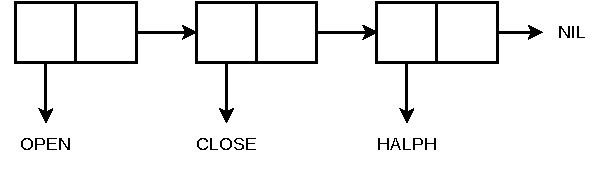
\includegraphics[width=0.8\textwidth]{img/list1.pdf}
\end{center}

\newpage

% 2. '((open1)(close2)(halph3))
\item '((open1)(close2)(halph3))
\begin{center}
    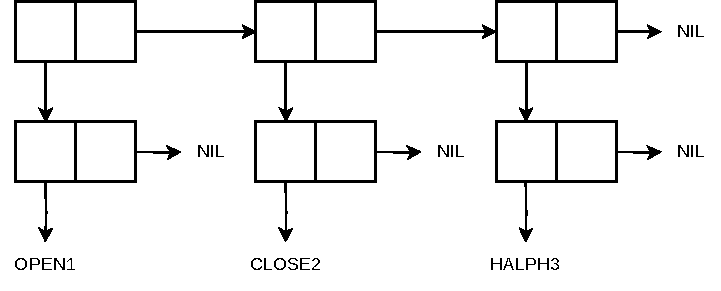
\includegraphics[width=0.9\textwidth]{img/list2.pdf}
\end{center}

% 3. '((one) for all (and (me (for you))))
\item '((one) for all (and (me (for you))))

См. Рисунок \ref{fig:3} в приложении А.

% 4. '((TOOL)(call))
\item '((TOOL)(call))
\begin{center}
    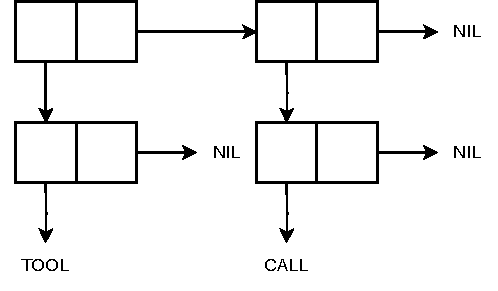
\includegraphics[width=0.65\textwidth]{img/list4.pdf}
\end{center}

\newpage

% 5. '((TOOL1)((call2))((sell)))
\item '((TOOL1)((call2))((sell)))
\begin{center}
    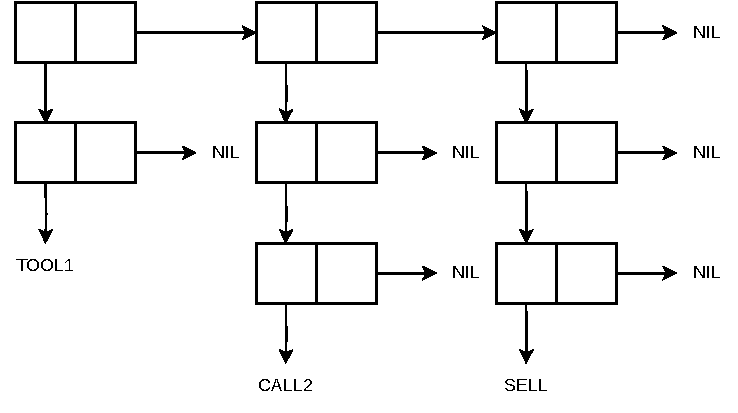
\includegraphics[width=0.9\textwidth]{img/list5.pdf}
\end{center}

% 6. '(((TOOL)(call))((sell)))
\item '(((TOOL)(call))((sell)))
\begin{center}
    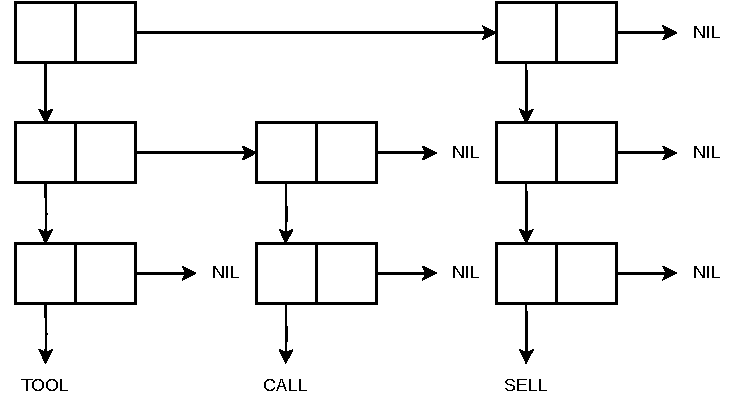
\includegraphics[width=0.9\textwidth]{img/list6.pdf}
\end{center}
\end{enumerate}

% \begin{lstlisting}[label={lst:}]
% 1) '(open close halph)
% 2) '((open1)(close2)(halph3))
% 3) '((one) for all (and (me (for you))))
% 4) '((TOOL)(call))
% 5) '((TOOL1)((call2))((sell)))
% 6) '(((TOOL)(call))((sell)))
% \end{lstlisting}

\newpage
\subsection{Задание 2}

Используя только функции CAR и CDR, написать выражения, возвращающие
\begin{enumerate}
    \item второй,
    \item третий,
    \item четвертый
\end{enumerate}
элементы заданного списка L.

\subsubsection*{Решение}

\begin{enumerate}
    \item Выражение, возвращающее второй элемент L:
        \begin{lstlisting}[label={lst:}]
(car (cdr L))
        \end{lstlisting}
    \item Выражение, возвращающее третий элемент L:
        \begin{lstlisting}[label={lst:}]
(car (cdr (cdr L)))
        \end{lstlisting}
    \item Выражение, возвращающее четвертый элемент L:
        \begin{lstlisting}[label={lst:}]
(car (cdr (cdr (cdr L))))
        \end{lstlisting}
\end{enumerate}

\newpage
\subsection{Задание 3}

Что будет в результате вычисления выражений?

\begin{enumerate}
    \item \begin{lstlisting}[label={lst:}]
(CAADR '((blue cube)(red pyramid)))
        \end{lstlisting}

    \item \begin{lstlisting}[label={lst:}]
(CDAR '((abc)(def)(gji))))
        \end{lstlisting}

    \item \begin{lstlisting}[label={lst:}]
(CADR '((abc)(def)(ghi)))
        \end{lstlisting}

    \item \begin{lstlisting}[label={lst:}]
(CADDR '((abc)(def)(ghi)))
        \end{lstlisting}
\end{enumerate}

% \newpage
\subsubsection*{Решение}

\begin{enumerate}
    \item Результат выполнения (CAADR '((blue cube)(red pyramid))) --- RED;
    \item Результат выполнения (CDAR '((abc)(def)(ghi)))) --- NIL;
    \item Результат выполнения (CADR '((abc)(def)(ghi))) --- DEF;
    \item Результат выполнения (CADDR '((abc)(def)(ghi))) --- GHI.
\end{enumerate}

\newpage
\subsection{Задание 4}

Напишите результат вычисления выражений и объясните, как он получен:

\begin{enumerate}
    \item \begin{lstlisting}[label={lst:}]
(list 'Fred 'and 'Wilma)
        \end{lstlisting}

    \item \begin{lstlisting}[label={lst:}]
(list 'Fred '(and Wilma))
        \end{lstlisting}

    \item \begin{lstlisting}[label={lst:}]
(cons Nil Nil)
        \end{lstlisting}

    \item \begin{lstlisting}[label={lst:}]
(cons T Nil)
        \end{lstlisting}

    \item \begin{lstlisting}[label={lst:}]
(cons Nil T)
        \end{lstlisting}

    \item \begin{lstlisting}[label={lst:}]
(list Nil)
        \end{lstlisting}

    \item \begin{lstlisting}[label={lst:}]
(cons '(T) Nil)
        \end{lstlisting}

    \item \begin{lstlisting}[label={lst:}]
(list '(one two) '(free temp))
        \end{lstlisting}

    \item \begin{lstlisting}[label={lst:}]
(cons 'Fred '(and Wilma))
        \end{lstlisting}

    \item \begin{lstlisting}[label={lst:}]
(cons 'Fred '(Wilma))
        \end{lstlisting}

    \item \begin{lstlisting}[label={lst:}]
(list Nil Nil)
        \end{lstlisting}

    \item \begin{lstlisting}[label={lst:}]
(list T Nil)
        \end{lstlisting}

    \item \begin{lstlisting}[label={lst:}]
(list Nil T)
        \end{lstlisting}

    \item \begin{lstlisting}[label={lst:}]
(cons T (list Nil))
        \end{lstlisting}

    \item \begin{lstlisting}[label={lst:}]
(list '(T) Nil)
        \end{lstlisting}

    \item \begin{lstlisting}[label={lst:}]
(cons '(one two) '(free temp))
        \end{lstlisting}
\end{enumerate}

\subsubsection*{Решение}

\begin{enumerate}
    \item 
        Выражение: (list 'Fred 'and 'Wilma);

        Аргументы list:
        \begin{itemize}
            \item Fred,
            \item and,
            \item Wilma;
        \end{itemize}

        Результат вычисления: (FRED AND WILMA);

        Объяснение: Функция list всегда возвращает список из своих аргументов. В данном выражении ей были переданны аргументы Fred, and и Wilma.

    \item 
        Выражение: (list 'Fred '(and Wilma));

        Аргументы list:
        \begin{itemize}
            \item Fred,
            \item (and Wilma);
        \end{itemize}

        Результат вычисления: (FRED (AND WILMA));

        Объяснение:
        % Функция list всегда возвращает список из своих аргументов. 
        В данном выражении list были переданны аргументы Fred и (and Wilma).

    \item 
        Выражение: (cons Nil Nil);

        Результат вычисления: (NIL);

        Объяснение: Функция cons принимает два аргумента, и возвращает точечную пару или списковую ячейку, в которой указатель CAR указывает на первый аргумент, а указатель CDR --- на второй аргумент. В данном выражении cons были переданны аргументы Nil и Nil, в результате чего была возвращена списковая ячейка, в которой указатели CAR и CDR указывают на Nil, а (Nil . Nil) эквивалентно (Nil).

    \item 
        Выражение: (cons T Nil);

        Результат вычисления: (T);

        Объяснение: В данном выражении cons были переданны аргументы T и Nil, в результате чего была возвращена списковая ячейка, в которой указатель CAR указывает на T, а указатель CDR --- на Nil. (T . Nil) эквивалентно (T).

    \item 
        Выражение: (cons Nil T);

        Результат вычисления: (NIL . T);

        Объяснение: В данном выражении cons были переданны аргументы Nil и T, в результате чего была возвращена точечная пара, в которой указатель CAR указывает на Nil, а указатель CDR --- на T.

    \item 
        Выражение: (list Nil);

        Аргументы list:
        \begin{itemize}
            \item Nil;
        \end{itemize}

        Результат вычисления: (NIL);

        Объяснение: В данном выражении list был передан только один аргумент --- Nil, следовательно, в результате вычисления выражения был создан список из одного элемента (Nil).

    \item 
        Выражение: (cons '(T) Nil);

        Результат вычисления: ((T));

        Объяснение: В данном выражении cons были переданны аргументы (T) и Nil, в результате чего была возвращена списковая ячейка, в которой указатель CAR указывает на список (T), состоящий из одного элемента (T), а указатель CDR --- на Nil. ((T) . Nil) эквивалентно ((T)).

    \item 
        Выражение: (list '(one two) '(free temp));

        Аргументы list:
        \begin{itemize}
            \item (one two),
            \item (free temp);
        \end{itemize}

        Результат вычисления: ((ONE TWO) (FREE TEMP));

        Объяснение: В данном выражении list были переданны аргументы (one two) и (free temp).

    \item 
        Выражение: (cons 'Fred '(and Wilma));

        Результат вычисления: (FRED AND WILMA);

        Объяснение: В данном выражении cons были переданны аргументы Fred и (and Wilma), в результате чего была возвращена списковая ячейка, в которой указатель CAR указывает на Fred, а указатель CDR --- на список (and Wilma), состоящий из двух списковых ячеек, в котором в первой ячейке указатель CAR указывает на and, а CDR --- на список (Wilma), в котором указатель CAR указывает на Wilma, а CDR --- на Nil. (Fred . (and Wilma)) эквивалентно (Fred and Wilma).

    \item 
        Выражение: (cons 'Fred '(Wilma));

        Результат вычисления: (FRED WILMA);

        Объяснение: В данном выражении cons были переданны аргументы Fred и (Wilma), в результате чего была возвращена списковая ячейка, в которой указатель CAR указывает на Fred, а указатель CDR --- на список (Wilma), в котором указатель CAR указывает на Wilma, а CDR --- на Nil. (Fred . (Wilma)) эквивалентно (Fred Wilma).

    \item 
        Выражение: (list Nil Nil);

        Аргументы list:
        \begin{itemize}
            \item Nil,
            \item Nil;
        \end{itemize}

        Результат вычисления: (NIL NIL);

        Объяснение: В данном выражении list были переданны два аргумента: Nil и Nil.

    \item 
        Выражение: (list T Nil);

        Аргументы list:
        \begin{itemize}
            \item T,
            \item Nil;
        \end{itemize}

        Результат вычисления: (T NIL);

        Объяснение: В данном выражении list были переданны аргументы T и Nil.

    \item 
        Выражение: (list Nil T);

        Аргументы list:
        \begin{itemize}
            \item Nil,
            \item T;
        \end{itemize}

        Результат вычисления: (NIL T);

        Объяснение: В данном выражении list были переданны аргументы Nil и T.

    \item 
        Выражение: (cons T (list Nil));

        Результат вычисления: (T NIL);

        Объяснение: При вычислении выражений в языке Lisp сначала вычисляются их аргументы. В результате вычисления T будет получено T. В результате вычисления (list Nil) будет получен список (NIL) из одного элемента --- Nil. В результате вычисления (cons T (NIL)) будет получена списковая ячейка, в которой указатель CAR указывает на T, а указатель CDR --- на список (Nil), в котором указатели CAR и CDR указывают на Nil. (T . (NIL)) эквивалентно (T NIL).

    \item 
        Выражение: (list '(T) Nil);

        Аргументы list:
        \begin{itemize}
            \item (T),
            \item Nil;
        \end{itemize}

        Результат вычисления: ((T) NIL);

        Объяснение: В данном выражении list были переданны аргументы (T) и Nil.

    \item 
        Выражение: (cons '(one two) '(free temp));

        Результат вычисления: ((ONE TWO) FREE TEMP);

        Объяснение: В данном выражении cons были переданны аргументы (one two) и (free temp), в результате чего была возвращена списковая ячейка, в которой указатель CAR указывает на список (one two), а указатель CDR --- на список (free temp).

\end{enumerate}

\newpage
\subsection{Задание 5}

Написать лямбда-выражение и соответствующую функцию:
\begin{enumerate}
    \item Написать функцию (f ar1 ar2 ar3 ar4), возвращающую список ((ar1 ar2) (ar3 ar4)).
    \item Написать фукнцию (f ar1 ar2), возвращающую ((ar1) (ar3)).
    \item Написать функцию (f ar1), возвращающую (((ar1))).
    \item Представить результаты в виде списочных ячеек.
\end{enumerate}

\subsubsection*{Решение}
\begin{enumerate}
    \item Функция: \begin{lstlisting}[label={lst:}]
(defun f (ar1 ar2 ar3 ar4) (cons (cons ar1 (cons ar2 nil)) (cons (cons ar3 (cons ar4 nil)) nil)))
        \end{lstlisting}
        Лямбда-выражение: \begin{lstlisting}[label={lst:}]
(lambda (ar1 ar2 ar3 ar4) (cons (cons ar1 (cons ar2 nil)) (cons (cons ar3 (cons ar4 nil)) nil)))
        \end{lstlisting}

    \item Функция: \begin{lstlisting}[label={lst:}]
(defun f (ar1 ar2) (cons (cons ar1 nil) (cons (cons ar2 nil) nil)))
        \end{lstlisting}
        Лямбда-выражение: \begin{lstlisting}[label={lst:}]
(lambda (ar1 ar2) (cons (cons ar1 nil) (cons (cons ar2 nil) nil)))
        \end{lstlisting}

    \item Функция: \begin{lstlisting}[label={lst:}]
(defun f (ar1) (cons (cons (cons ar1 nil) nil) nil))
        \end{lstlisting}
        Лямбда-выражение: \begin{lstlisting}[label={lst:}]
(lambda (ar1) (cons (cons (cons ar1 nil) nil) nil))
        \end{lstlisting}

        \newpage
    \item Представление результатов в виде списковых ячеек:
\end{enumerate}

\begin{center}
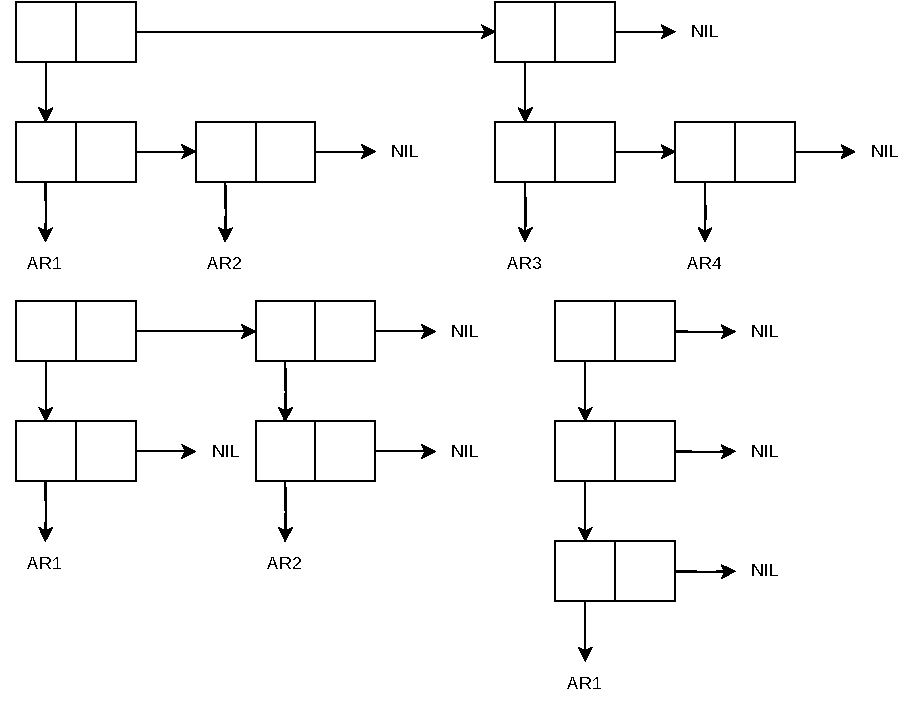
\includegraphics[width=\textwidth]{img/task5.pdf}
\end{center}

\newpage
% \section*{Теоретические вопросы}
\section{Теоретические вопросы}

\subsection{Элементы языка}

\begin{figure}[H]
	\centering
    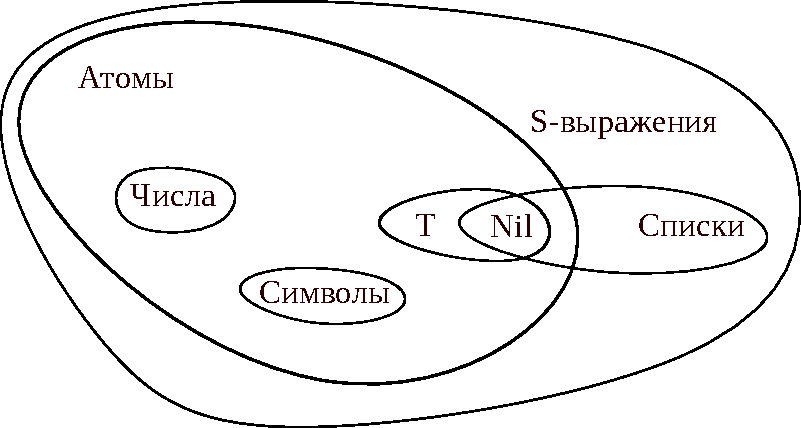
\includegraphics[width=0.9\textwidth]{img/lisp.pdf}
	\caption{Элементы языка Lisp}
	\label{fig:lisp}
\end{figure}

Вся информация (данные и программы) в Lisp представляются в виде символьных выражений --- S-выражений. По определению

{S-выражение ::= <атом> | <точечная пара>}.

\noindent Элементарные значения структур данных:

Атомы:
\begin{itemize}
    \item символы (идентификаторы) --- синтаксически --- набор литер (букв и цифр), начинающихся с буквы;
    \item специальные символы --- \{T, Nil\} (используются для обозначения логических констант);
    \item самоопределимые атомы --- натуральные числа, дробные числа (например, 2/3), вещественные числа, строки --- последовательность символов, заключенных в двойные апострофы (например, ``abc'');
\end{itemize}

Более сложные данные --- списки и точечные пары (структуры) строятся из унифицированных структур --- блоков памяти --- бинарных узлов.

\subsubsection{Определения}

Точечные пары ::= (<атом>.<атом>) | ((<атом>.<точечная пара>) | (<точечная пара>.<атом>) | (<точечная пара>.<точечная пара>);

Список ::= <пустой список> | <непустой список>, где

<пустой список> ::= () | Nil,

<непустой список> ::= (<первый элемент>.<хвост>),

<первый элемент> ::= <S-выражение>,

<хвост> :: <список>.

\subsubsection{Синтаксис}

Любая структура (точечная пара или список) заключается в круглые скобки.
(A.B) --- точечная пара, (A) --- список из одного элемента).
Пустой список изображается как Nil или (); непустой список по определению может быть изображен: (A.(B.(C.(D())))), допустимо изображение списка последовательностью атомов, разделенных пробелами --- (A B C D).

Элементы списка могут, в свою очередь, быть списками (любой список заключается в круглые скобки), например --- (A (B C) (D (E))).

Таким образом, синтаксически наличие скобок является признаком структуры --- списка или точечной пары.

\subsubsection{Представление в памяти}

Любая непустая структура Lisp в памяти представляется списковой ячейкой, хранящей два указателя: на голову (первый элемент) и хвост --- все остальное.

\subsection{Особенности языка Lisp. Структура программы}

\begin{itemize}
    \item В лиспе программист описывает то, что он хочет получить;
    % \item В лиспе используется нотация Черча, то есть, 5 --- это (+ 1 (+ 1 (+ 1 (+ 1 (+ 1 0))))) --- фукнция от нуля аргументов;
    \item В лиспе функция всегда возвращает какое-то значение;
    \item Лисп опирается на лямбда-исчисление Черча: все действия, которые можно выполнить, можно организовать в виде функций;
    \item Малое количество констркуций языка дает много возможностей;
    \item Поддерживается символьная обработка данных, в связи с чем можно писать программы, изменяющие собственный код в процессе выполнения;
    \item Лисп --- безтиповый язык без операторов с автоматическим управлением памятью;
    \item Память выделяется блоками, всегда одинаковыми; блок памяти --- списковая ячейка ячейка (два указателя).
\end{itemize}

% \subsection{Структура программы}

\subsection{Символ апостроф}

Символ апостроф --- сокращенное обозначение функции quote.
Можно считать, что апостроф <<блокирует>> вычисления.

\subsection{Базис языка Lisp. Ядро языка}

Базис языка Lisp --- минимальный набор конструкций языка и структур данных, с помощью которого можно написать любую программу.

Базис языка Lisp включает атомы, бинарные узлы (для представления структур), базовые функции и функционалы.

% \subsection{Ядро языка}

% -------------------------------------------------------------------

\newpage
\phantomsection\section*{ПРИЛОЖЕНИЕ А}\addcontentsline{toc}{section}{ПРИЛОЖЕНИЕ А}

\begin{figure}[H]
	\centering
    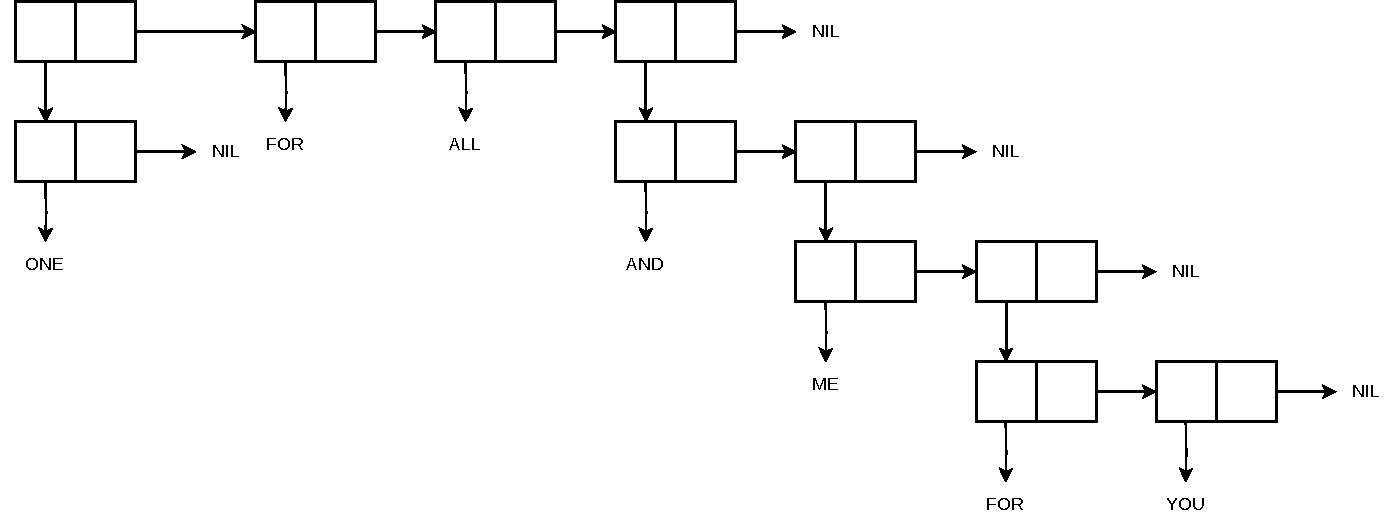
\includegraphics[angle=90, height=0.8\textheight]{img/list3.pdf}
	\caption{'((one) for all (and (me (for you))))}
	\label{fig:3}
\end{figure}

\end{document}
